\chapter{Kernel Configuration}

In this chapter the working with the Linux kernel is described. There are some tutorials from the supervisor on GitHub, which can be found here: \url{https://github.com/dasGringuen/MicroZedKernel}\newline
The Kernel Sources are needed to develop a module for this Kernel. The sources contain all the Header files for the module. After compiling the Kernel the Device Tree has to be adjusted. The Device Tree handles the Hardware, and replaces the BIOS. After finishing this steps the Driver Development can be started.

\subsection{First Stage Boot loader}

Before the SPI on the MicroZed Board can be used, the FPGA has to be programmed. The Bitstream for the Programming is a standard pattern in the Vivado tool chain. The following picture shows the Configuration of the SPI in the Vivado:

\begin{figure}[H]
	\centering
		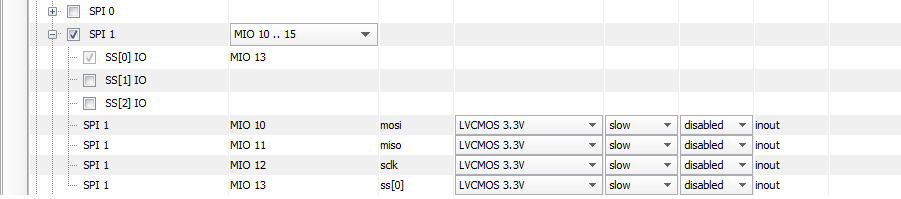
\includegraphics[width=1.00\textwidth]{picture/Pin_setup.png}
	\caption{Vivado SPI pinout}
	\label{fig:rfm12}
\end{figure}

The same Bitstream can be used for the Linux module and the Bare-metal program. The first attempt for loading the Bitstream was to start Linux and simply program the FPGA with the internal driver: \verb|cat bitstream.bit > /dev/xdevcfg|. This is working very easy and can be extended with the crontab program to program the FPGA after start-up. Therefore this simple line has to be added to crontab:\verb|@reboot cat /root/system_wrapper.bit > /dev/xdevcfg|. To configure crontab the following call can be used: \verb|crontab -e|\newline

\emph{But this is not working with the SPI}. While the System is booting it checks if the desired Hardware is available in the FPGA. So the OS thinks there is a SPI, but it is not in the FPGA. It just appears after the start-up. The Solution for this is to program the FPGA before the u-boot Bootloader loads the Linux in the RAM. Therefore the MicroZed Board has 2 Bootloader. The First Stage Bootloader can program the FPGA and after that he is loading the u-boot which is loading the Linux. The First Stage Bootloader can easily be created with the SDK of Xilinx. An step by step instruction can be fund on GitHub \url{https://github.com/SchoAr/RFM12_Linux/blob/master/FSBL/how_to_create_fslb.txt}\newline
Important is that the Board Support Package of the First stage Bootloader contains the SPI. Otherwise the programming might not work. The U-boot Image can be downloaded from Xilinx. A compiled version can also be found on GitHub. After compiling the Bootloader it is simply copied on the SD Card. 

\subsection{Device tree}

As described before the Device tree contains the hardware which is available via the Linux. The File which contains the Device tree can be found in the following directory:\newline\verb|./arch/arm/boot/dts/zynq-7000.dtsi|. In the predefined Device tree the SPI is not enabled. The SPI1 is simply enabled by deleting the "disable" status. The Following code shows this:

\begin{lstlisting}
spi1: spi@e0007000 {
					compatible = "xlnx,zynq-spi-r1p6";
          reg = <0xe0007000 0x1000>;
-         status = "disabled";   						//Delete this
          interrupt-parent = <&intc>;
          interrupts = <0 49 4>;
          clocks = <&clkc 26>, <&clkc 35>;
    }                                                                                                                           
\end{lstlisting}

Now we need to add in the settings the SPI Configuration this is done in the following file:\newline\verb| ./arch/arm/boot/dts/zynq-zed.dts|. Here are the parameters for the devices saved. Here the SPI1 has to be added to use it for the Driver. The following listing shows the code,which has to be added:
\begin{lstlisting}
+&spi1 {
+        status = "okay";
+        num-cs = <4>;
+        is-decoded-cs = <0>;
+};
\end{lstlisting}

It is also possible to add a specific device to the device tree which can then be used in user space. The following listing shoes this example. If this is applied a SPI master device will appear in /dev. With a simple echo command it is possible to send Data. This is good practice if it is necessary to test the SPI without writing a Module. This has been done to check if the first stage Bootloader loaded successful the Bitstream in the FPGA.

\begin{lstlisting}
&spi1 {
       status = "okay";
       num-cs = <4>;
       is-decoded-cs = <0>;
       device@2 {
                compatible = "spidev";
                reg = <0>;
                spi-max-frequency = <500000>;
                };            
};
\end{lstlisting}



